\newpage
\section{Conduite du projet}
\subsection{Tableau Trello sprint 1}
Lors du premier sprint (le 8 mars 2021), la visualisation de carte ainsi que la visualisation de carte avec contrainte était en cours alors que le bouton "play!", la sélection du niveau de questions , le bouton "exit", une alerte de confirmation 
de la réponse ainsi que le menu pour ajouter une carte était déjà prête. 
Il restait encore énormement de travail.

\begin{figure}[h]
	\centering
	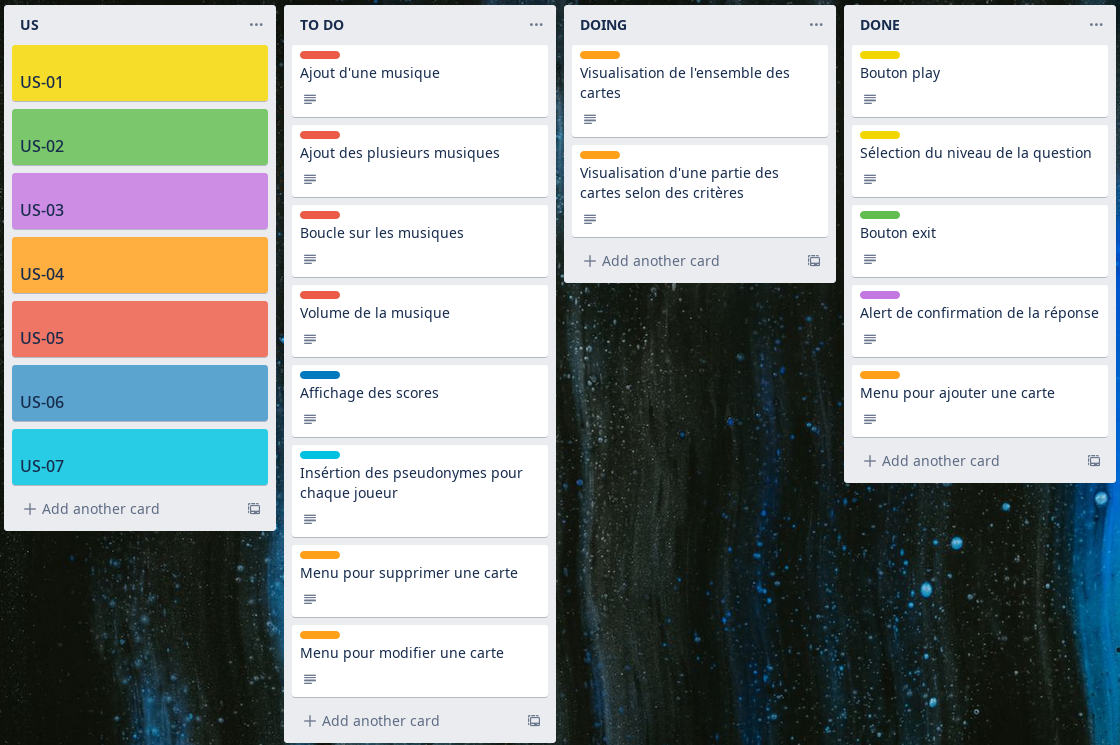
\includegraphics[width=\textwidth]{trello1.png}
	\caption{Tableau Trello sprint 1}
	\label{fig:Trello_sprint_1}
\end{figure}

\newpage
\subsection{Tableau Trello sprint 2}
Lors du deuxième sprint (le 29 mars 2021),  la fênetre des paramètre ainsi que ses premiers composants (volume musique, le bouton "mute") était en cours de codage tandis que l'affichage des scores, les menus de modification et de suppression de 
carte, l'ajout de la musique , la playlist musicale ainsi que l'utilisation de pseudo encoder par l'utilisateur avait été terminé.
Le projet avançait à bon pas et la base du projet était quasi fini. 

\begin{figure}[h]
	\centering
	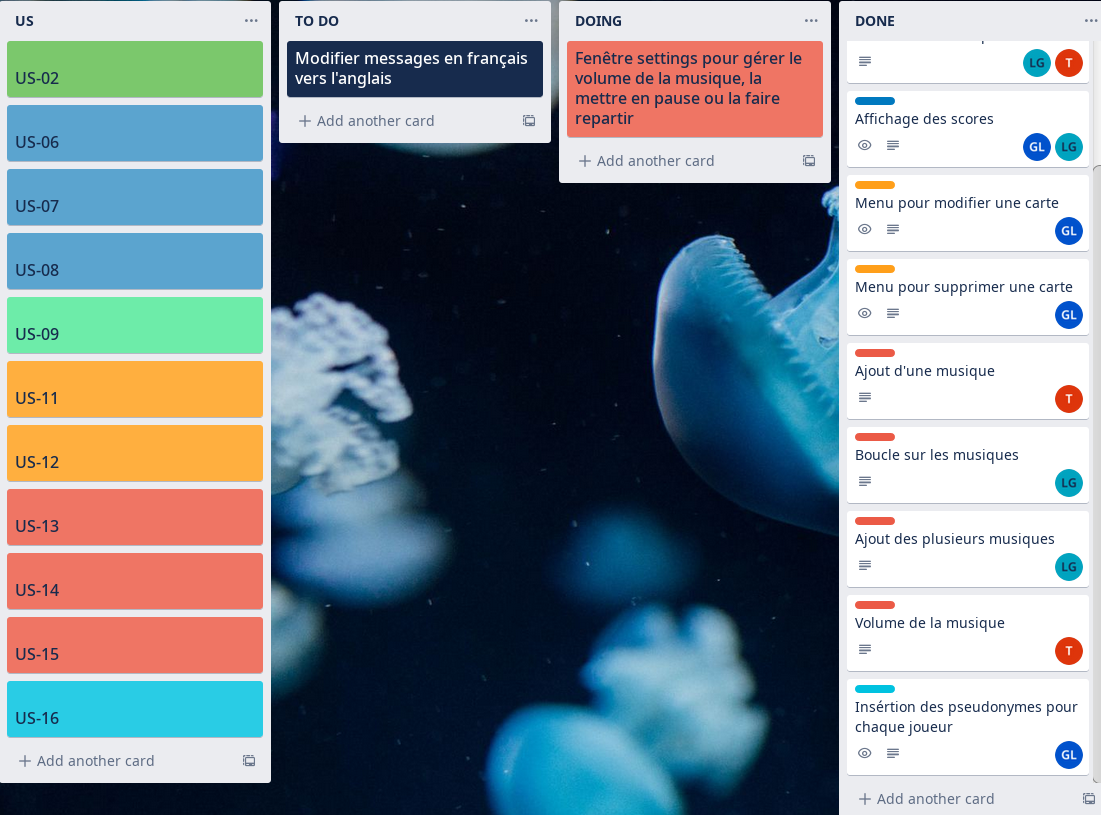
\includegraphics[width=\textwidth]{trello2.png}
	\caption{Tableau Trello sprint 2}
	\label{fig:Trello_sprint_2}
\end{figure}

\newpage
\subsection{Tableau Trello sprint 3}
Concernant le troisième sprint (le 26 avril 2021), il ne reste plus que la mise en place de la partie multijoueur en ligne.
La fenêtre des paramètres ainsi que la création d'un menu pause ont été terminer. 
Le plateau de jeu ainsi que les pions ont également été fait durant ce sprint.
Bien que le mode multi joueur en ligne ne sois pas terminé, les possibilité d'héberger ou de rejoindre une partie ainsi qu'un chat ont été terminer.

\begin{figure}[h]
	\centering
	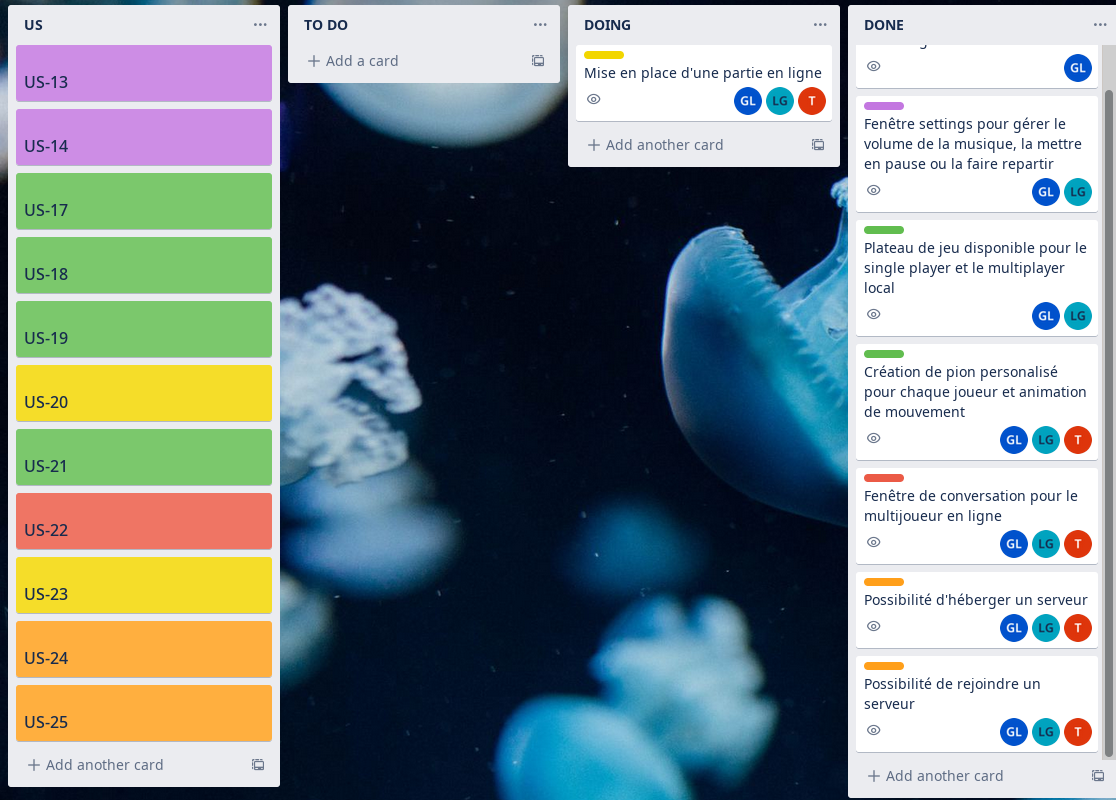
\includegraphics[width=\textwidth]{trello3.png}
	\caption{Tableau Trello sprint 3}
	\label{fig:Trello_sprint_3}
\end{figure}